\section{Wielomian Jonesa} % (fold)
\label{sec:jones}

Znamy już jeden wielomianowy niezmiennik splotów, odkryty przez Alexandera w~latach dwudziestych ubiegłego wieku.
Blisko czterdzieści lat później John Conway znalazł prosty sposób na wyznaczenie wielomianu
Alexandera dla każdego splotu przy użyciu tak zwanej relacji kłębiastej (\emph{,,skein relation''}):
jest ona prostym równaniem wiążącym wielomian splotu oraz wielomiany
splotów o~zmodyfikowanych pojedynczych skrzyżowaniach (na diagramie).
Narzędzie to okazało się być kluczem do sukcesu.

Vaughan Jones, matematyk nowozelandzki, zaprezentował w~roku 1984 nowy niezmiennik splotów
jako produkt uboczny podczas pracy nad algebrami operatorowymi, które nas nie interesują.
Był to przełomowy rezultat, a~już cztery miesiące później ogłoszono znalezienie
jeszcze bardziej wyrafinowanego niezmiennika, któremu przyjrzymy się w~kolejnej sekcji.

Aby lepiej zrozumieć wielomian Jonesa, zbadamy najpierw nieco prostszy obiekt, nawias Kauffmana.
Później zajmiemy się węzłami alternującymi.

\subsection{Nawias Kauffmana} % (fold)
\label{sub:kauffman_bracket}
Zaczniemy od zdefiniowania nawiasu Kauffmana.
Przypomnijmy, wielomian Laurenta zmiennej $X$ to formalny symbol $f=a_r X^r + \ldots + a_s X^s$,
gdzie $r, s, a_r, \ldots, a_s$ są całkowite i $r \le s$.

Poszukujemy niezmiennika dla splotów o kilku prostych własnościach.
Przede wszystkim żądamy,
by niewęzłowi przypisany był wielomian $1$: $\bracket{\LittleUnknot} = 1$.
Po drugie chcemy wyznaczać nawiasy znając je dla prostszych splotów,
co zapiszemy symbolicznie $\bracket{\LittleRightCrossing} = A \bracket{\LittleRightSmoothing} + B \bracket{\LittleLeftSmoothing}$.
Zależy nam wreszcie na tym, by móc dodać do splotu trywialną składową:
$\langle L \cup \LittleUnknot \rangle = C \langle L \rangle$.

Prosty rachunek pokazuje wpływ drugiego ruchu Reidemeistera na nawias:
\[
    \bracket{\reidemeisterIIaa}
    = (A^2 + ABC + B^2) \bracket{\LittleLeftSmoothing} + BA \bracket{\LittleRightSmoothing}
    \stackrel{?}{=} \bracket{\LittleRightSmoothing}.
\]

Aby zachodziła ostatnia równość wystarczy (chociaż wcale nie trzeba) przyjąć
$B = A^{-1}$, co wymusza na nas $C = -A^2 - A^{-2}$.
W ten sposób odkryliśmy następującą definicję.

\begin{definition}[nawias Kauffmana]
    \index{nawias!Kauffmana}
    Wielomian Laurenta $\bracket{D}$ dla diagramu splotu $D$ zmiennej $A$,
    który jest niezmienniczy ze względu na gładkie deformacje diagramu,
    a przy tym spełnia trzy poniższe aksjomaty, to nawias Kauffmana.
    \begin{align}
        \bracket{\LittleUnknot} & = 1 \\
        \bracket{D \sqcup \LittleUnknot} & = (-A^{-2} - A^2) \bracket{D} \\
        \bracket{\LittleRightCrossing} & = A \bracket{\LittleRightSmoothing} + A^{-1} \bracket{\LittleLeftSmoothing}
    \end{align}
\end{definition}

Tutaj $\LittleUnknot$ oznacza standardowy diagram dla niewęzła,
zaś trzy symbole $\LittleRightCrossing$, $\LittleRightSmoothing$ oraz $\LittleLeftSmoothing$ odnoszą się do diagramów,
które są identyczne wszędzie poza małym obszarem (tak jak w relacji kłębiastej).

Diagramy $\LittleRightSmoothing$ oraz $\LittleLeftSmoothing$ nazywa się odpowiednio
dodatnim (prawym) i ujemnym (lewym) wygładzeniem $\LittleRightCrossing$.

\begin{lemma}
    Nawias Kauffmana każdego diagramu wyznacza się w skończenie wielu krokach.
\end{lemma}

\begin{proof}
    Jeżeli diagram $D$ ma $n$ skrzyżowań, to nieustanne stosowanie aksjomatu trzeciego pozwala na zapisanie $\bracket{D}$ jako sumy $2^n$ składników,
    z których każdy jest po prostu zamkniętą krzywą i ma trywialny nawias ($\bracket{\LittleUnknot} = 1$).
    Nawias sumy wyznacza się korzystając z drugiego aksjomatu.
\end{proof}

Przedstawimy teraz wpływ ruchów Reidemeistera na nawias Kauffmana.

\begin{lemma}
    Drugi i trzeci ruch Reidemeistera nie ma wpływu na klamrę Kauffmana,
    pierwszy ruch zmienia ją zgodnie z regułą:
    \[
        \bracket{\reidemeisterIa} = -A^{-3} \bracket{\,\reidemeisterIb\,}.
    \]
\end{lemma}

\begin{proof}
Pierwszy ruch Reidemeistera:
\[
    \bracket{\reidemeisterIa} \stackrel{K3}{=} A \bracket{
    \begin{tikzpicture}[baseline=-0.65ex,scale=0.07]
    \useasboundingbox (-4, -5) rectangle (3, 5);
    \begin{knot}[clip width=5, end tolerance=1pt]
        \strand[semithick]
            (-3, 5) [in=left, out=down] to (-1,1) [in=left, out=right]
                                        to (1,3)
                                        to [in=up, out=right] (3,0);
        \strand[semithick]
            (-3, -5) [in=left, out=up] to (-1,-1) [in=left, out=right]
                                       to (1, -3)
                                       to [in=down, out=right] (3,0);
    \end{knot}
    \end{tikzpicture}}
    + A^{-1} \bracket{\,
    \begin{tikzpicture}[baseline=-0.65ex,scale=0.07]
    \begin{knot}[clip width=5]
        \strand[semithick] (0,-5) [in=down, out=up] to (1, -2) to (1, 2) to (0, 5);
        \strand[semithick] (4,0) circle (1.5);
    \end{knot}
    \end{tikzpicture}}
    \stackrel{K2}{=} A \bracket{\,\reidemeisterIb\,} + A^{-1}(-A^{-2}-A^2) \bracket{\,\reidemeisterIb\,}
    = -A^{-3}\bracket{\,\reidemeisterIb\,}
\]

Pierwsza równość wynika z $K3$, druga z $K2$, trzecia jest oczywista.
Dla drugiego ruchu:
\begin{align*}
    \bracket{\reidemeisterIIa} &\stackrel{K3}{=} A
    \bracket{\reidemeisterIab}
    + A^{-1} \bracket{\begin{tikzpicture}[baseline=-0.65ex,scale=0.07]
    \useasboundingbox (-5, -6) rectangle (5, 6);
    \begin{knot}[clip width=5, end tolerance=1pt]
        \strand[semithick] (4,-5) .. controls (4,-2) and (-4,-2) .. (-4,0);
        \strand[semithick] (4,5) to (4,0);
        \strand[semithick] (-4,-5) .. controls (-4,-2) and (4,-2) .. (4,0);
        \strand[semithick] (-4,5) to (-4,0);
    \end{knot}
    \end{tikzpicture}}
    \stackrel{K1}{=} -A^{-2} \bracket{\LittleLeftSmoothing} + A^{-1}
    \bracket{\begin{tikzpicture}[baseline=-0.65ex,scale=0.07]
    \useasboundingbox (-5, -6) rectangle (5, 6);
    \begin{knot}[clip width=5, end tolerance=1pt]
        \strand[semithick] (4,-5) .. controls (4,-2) and (-4,-2) .. (-4,0);
        \strand[semithick] (4,5) to (4,0);
        \strand[semithick] (-4,-5) .. controls (-4,-2) and (4,-2) .. (4,0);
        \strand[semithick] (-4,5) to (-4,0);
    \end{knot}
    \end{tikzpicture}}
    \\ & \stackrel{K3}{=} -A^{-2} \bracket{\LittleLeftSmoothing}
    + A^{-1}A \bracket{\LittleRightSmoothing} + A^{-1}A^{-1} \bracket{\LittleLeftSmoothing}
    = \bracket{\LittleRightSmoothing}
\end{align*}

Dla trzeciego ruchu:
\begin{align*}
\bracket{\,\reidemeisterIIIa\,} &\stackrel{K3}{=} A
\bracket{\,\begin{tikzpicture}[baseline=-0.65ex,yscale=0.07, xscale=0.1]
    \useasboundingbox (-5, -6) rectangle (5, 6);
    \begin{knot}[clip width=5, flip crossing/.list={1,2,3}, end tolerance=1pt]
        \strand[semithick] (-5, 5) [in=-135, out=-45] to (5,5);
        \strand[semithick] (-5, -5) [in=135, out=45] to (5,-5);
        \strand[semithick] (-5, 0) .. controls (-2, 0) and (-2,5) .. (0,5) .. controls (2, 5) and (2, 0) .. (5, 0);
    \end{knot}
    \end{tikzpicture}\,}
+A^{-1} \bracket{\RightCrossSmoothing} \\
%\stackrel{R2}{=} A \bracket{\,\LeftCrossSmoothing\,} +A^{-1} \bracket{\RightCrossSmoothing} \\
& \stackrel{R2}{=} A \bracket{\,\LeftCrossSmoothing\,} +A^{-1} \bracket{\RightCrossSmoothing}
\stackrel{K3}{=} \bracket{\,\reidemeisterIIIb\,}
\end{align*}
korzystaliśmy tu z własności drugiego ruchu.
\end{proof}

Zaniechamy ratowania niezmienniczości nawiasu Kauffmana na ruchy Reidemeistera, zamiast tego przejdziemy do kolejnego składnika w przepisie na wielomian Jonesa.
Prostym wnioskiem z lematu jest niezmienniczość rozpiętości (różnicy pomiędzy najwyższym oraz najniższym wykładnikiem) nawiasu.

Gregor Schaumann w notatkach \cite{schaumann16} wprowadza rachunek schematyczny,
który pozwala spojrzeć na nawias Kauffmana z nowej perspektywy.
Definiuje kwantowe niezmienniki oraz plątaniny (równoważne wtedy,
kiedy związane są przez ciąg tożsamości wężowych, ruchów Turaewa oraz Reidemeistera).
Wspomniane są też dokonania Wasiljewa.
% Koniec podsekcji Nawias Kauffmana


\subsection{Spin} % (fold)
\label{sub:writhe}
Przypomnijmy, że znak skrzyżowania na diagramie to liczba $1$ lub $-1$ (definicja \ref{sign_def}).

\begin{definition}[spin]
    \index{spin}
    Wielkość
    \begin{equation}
        w(D) = \sum_c \operatorname{sign} c,
    \end{equation}
    gdzie sumowanie przebiega po wszystkich skrzyżowaniach diagramu $D$ zorientowanego splotu lub węzła, nazywamy spinem.
    Z angielskiego \emph{writhe}.
\end{definition}

Co ważne, spin nie jest niezmiennikiem splotów ani węzłów.
Para Perko przedstawia ten sam węzeł z~minimalną liczbą skrzyżowań i~spinem równym siedem lub dziewięć.
Dzięki temu przez wiele lat nie została dostrzeżona.
Spin jest za to niezmiennikiem węzłów alternujących, mówi o~tym druga hipoteza Taita.

\begin{lemma}
    Spin nie zależy od orientacji.
    Tylko I ruch Reidemeistera zmienia spin: $w(\MalyreidemeisterIa) = w(\MalyreidemeisterIb )-1$, pozostałe ruchy nie mają na niego wpływu.
\end{lemma}

%\begin{proof}
    %Proste ćwiczenie.
%\end{proof}

% Koniec sekcji Spin


\subsection{Wielomian Jonesa} % (fold)
\label{sub:jones}
\begin{definition}
	\index{wielomian!Jonesa}
	\emph{Wielomian Jonesa} zorientowanego splotu to wielomian Laurenta $V(L)\in\Z[t^{1/2},t^{-1/2}]$ określony przez
	\[
		V(L)=\left[(-A)^{-3w(D)} \bracket{D}\right]_{t^{1/2}=A^{-2}},
	\]
	gdzie $D$ to dowolny diagram dla $L$.
\end{definition}

Połączenie \emph{writhe} z nawiasem nazywamy ,,trikiem Kauffmana''.

\begin{proposition}
	Wielomian Jonesa jest niezmiennikiem zorientowanych splotów.
\end{proposition}

\begin{proof}
	%Skorzystamy z tego, że indeks zaczepienia jest niezmiennikiem.
	Wystarczy pokazać niezmienniczość $(-A)^{-3w(D)}\langle D\rangle$ na ruchy Reidemeistera.
	Ale
	\[
		(-A)^{-3 w\left(\MalyreidemeisterIa\right)} \bracket{\MalyreidemeisterIa} =
		(-A)^{-3 w\left(\ \MalyreidemeisterIb\ \right)+3} (-A)^{-3}\bracket{\ \MalyreidemeisterIb\ } =
		(-A)^{-3 w\left(\ \MalyreidemeisterIb\ \right)}	\bracket{\,\MalyreidemeisterIb\,}. \qedhere
	\]
\end{proof}

Wielomian Jonesa jest naprawdę potężnym narzędziem.
Pozwala bowiem odróżnić dowolne dwa węzły pierwsze o co najwyżej dziewięciu skrzyżowaniach.

\begin{conjecture} \label{jones_conjecture}
	Nie istnieje nietrywialny węzeł, którego wielomian Jonesa nie odróżnia od niewęzła.
\end{conjecture}

Istnieją sploty o trywialnym wielomianie Jonesa, jest ich nawet nieskończenie wiele, jak Eliahou, Kauffman i Thistlethwaite pokazali w pracy \cite{eliahou03}.
Argumentem przemawiającym za prawdziwością hipotezy jest twierdzenie udowodnione przez Jørgena Andersena.
Pokazał on, że rodzina okablowanych wielomianów Jonesa wykrywa niewęzeł.
Tutaj $n$-okablowanie węzła $K$ to $n$-komponentowy splot $K^n$, który powstaje z $K$ po zamianie pojedynczej ,,żyły'' na $n$ równoległych żył.
Hipotezę zweryfikowano dla węzłów o małej liczbie skrzyżowań metodami komputerowymi.
W latach dziewięćdziesiątych Hoste, Thistlethwaite, Weeks zrobili to dla węzłów spełniających $u \le 16$.
Wynik poprawiano: Dasbach, Hougardy w 1997 do $u = 17$; Yamada w 2000 do $u = 18$; wreszcie Tuzun, Sikora w 2016 do $u \le 22$.

Wartości wielomianu Jonesa w niektórych pierwiastkach jedności są związane z innymi niezmiennikami węzłów.
I tak przyjmując oznaczenie $\omega_n = \exp(2\pi i/n)$ mamy

\begin{proposition} \label{jones_sharp_p_hard}
	Niech $V$ będzie wielomianem Jonesa splotu $K$ o $n$ składowych spójności.
	Wtedy:
	\begin{compactenum}
		\item $V(1) = (-2)^{n-1}$;
		\item $V(-1)$ jest rzędem pierwszej grupy homologii podwójnego nakrycia $S^3$ rozgałęzionego nad składowymi, jeśli jest torsyjna; $V(-1) = 0$ w przeciwnym razie;
		\item $V(\omega_3) = 1$;
		\item $V(i) = (-\sqrt 2)^{n-1}(-1)^{\operatorname{Arf} K}$ jeśli $K$ jest właściwym splotem (indeks zaczepienia każdej składowej o resztę splotu jest parzysty), $V(i) = 0$ w przeciwnym razie;
		\item wielkość $3|V(\omega_6)|^2$ opisuje liczbę trzy-kolorowań splotu.
	\end{compactenum}
	Dla węzłów te zależności można uprościć: $V(1) = 1$; $V(-1) = \pm \det K$; $V(i) = 1$ jeśli $\Delta(-1)$ jest postaci $8k \pm 1$, w przeciwnym razie $V(i) = -1$.
\end{proposition}

\begin{proof}
	Równości 1. i 3. są prostym wnioskiem z relacji kłębiastej, patrz też \cite{jones87}.
	Dowód 5. zawiera praca ,,3-coloring and other elementary invariants of knots'' (Przytycki, 1998).
	Równość 4. pokazał Murakami w 1986 roku (\cite{murakami86}).
\end{proof}

Poza powyżej opisanymi przypadkami, wartości wielomianu Jonesa nie można znaleźć w czasie wielomianowym od ilości skrzyżowań na diagramie (jest to problem $\#P$-trudny).
Nie jest znana charakteryzacja wielomianu Jonesa poza warunkami koniecznymi z faktu \ref{jones_sharp_p_hard} ani jego topologiczna interpretacja (którą posiada wielomian Alexandera).

Czemu wielomian Jonesa jest wielomianem?
Odpowiedniki wielomianu Jonesa dla węzłów w 3-rozmaitościach innych niż sfera $S^3$ nie są wielomianami, ale funkcjami z pierwiastków jedności w zbiór elementów całkowitch\footnote{algebraic integers} (jak podaje J. Roberts).

% Koniec podsekcji Wielomian Jonesa


\subsection{Relacja kłębiasta} % (fold)
\label{sub:skein}
Dotychczas wyznaczyliśmy wielomian Jonesa jedynie dla trywialnych splotów.
Spowodowane jest to tym, że chociaż nawias Kauffmana jest przydatny przy dowodzeniu różnych własności,
to zupełnie nie nadaje się do obliczeń.
Dużo lepszym narzędziem jest następujące twierdzenie.

\begin{theorem}[relacja kłębiasta] \label{tracheotomia} \index{Relacja kłębiasta}
    Wielomian Jonesa spełnia równość $V(\LittleUnknot) = 1$ oraz relację
    \[
        t^{-1} V(L_+) - tV(L_-) + (t^{-1/2} - t^{1/2}) V(L_0) = 0,
    \]

    gdzie $L_+$, $L_-$, $L_0$ to zorientowane sploty, które różnią się jedynie na małym obszarze:
    \[
        \skeinplus \quad\quad\quad\quad
        \skeinminus \quad\quad\quad\quad
        \skeinzero
    \]
\end{theorem}

\begin{proof}
Wyraźmy wielomian Jonesa przez nawias Kauffmana i spin.
Chcemy pokazać, że
\[
    A^{4}(-A)^{-3w(L_+)}\bracket{\LittleRightCrossing}
    -A^{-4}(-A)^{-3w(L_-)}\bracket{\LittleLeftCrossing}
    +(A^2-A^{-2})(-A)^{-3w(L_0)}\bracket{\LittleRightSmoothing} = 0.
\]

Ale $w(L_\pm)=w(L_0)\pm 1$, zatem to jest równoważne z
\[
    -A\bracket{\LittleRightCrossing} +A^{-1}\bracket{\LittleLeftCrossing} +(A^2-A^{-2})\bracket{\LittleRightSmoothing} =0.
\]
Z definicji nawiasu Kauffmana wnioskujemy, że
$\bracket{\LittleRightCrossing} = A\bracket{\LittleRightSmoothing}+A^{-1}\bracket{\LittleLeftSmoothing}$ i
$\bracket{\LittleLeftCrossing} = A\bracket{\LittleLeftSmoothing}+A^{-1}\bracket{\LittleRightSmoothing}$.
Pierwsze równanie przemnóżmy przez $A$, drugie przez $A^{-1}$, a następnie dodajmy je do siebie.
Wtedy otrzymamy $A\bracket{\LittleRightCrossing}-A^{-1}\bracket{\LittleLeftCrossing} =
A^2\bracket{\LittleRightSmoothing} - A^{-2}\bracket{\LittleRightSmoothing}$.
\end{proof}
% Koniec sekcji Relacja kłębiasta


% \subsection{Odwrotności, lustra i sumy}
\begin{proposition}
    Niech $L$ będzie zorientowanym splotem.
    $V(rL)=V(L)$, $V(mL)(t)=V(L)(t^{-1})$.
\end{proposition}

\begin{proof}
    Aby obliczyć wielomian rewersu, wykorzystujemy te same diagramy kłębiaste,
    jak dla zwykłego, a przy tym nie zmieniamy znaku żadnego skrzyżowania.

    Druga część: Florian Gellert, Kombinatorische Invarianten, strona 12.
\end{proof}

\begin{corollary}
    Wielomian Jonesa nie zależy od orientacji węzła (ale nie splotu!).
\end{corollary}

\begin{proof}
    Każdy węzeł ma tylko dwie orientacje, splot może mieć ich $2^n$, gdzie $n$ to liczba składowych.
\end{proof}

\begin{proposition}
    Niech $L, M$ będą zorientowanymi splotami, zaś $J, K$: zorientowanymi węzłami.
    \begin{enumerate}
        \item $V(L \sqcup M) = (-t^{1/2} - t^{-1/2}) V(L) V(M)$,
        \item $V(J \# K) = V(J) V(K)$.
    \end{enumerate}
\end{proposition}

\begin{proof}
    Wybierzmy diagramy $D, E$ dla (odpowiednio) $L, M$.
    Po podstawieniu $t^{1/2}=A^{-2}$ widzimy, że chcemy pokazać
    $(-A)^{-3w(D\sqcup E)}\langle D\sqcup E\rangle =(-A^2-A^{-2})(-A)^{-3(w(D)+w(E))}\langle D\rangle  \langle E\rangle$.

    Oczywiście $w(D\sqcup E)=w(D)+w(E)$, więc wystarczy udowodnić, że
    \[
        \langle D\sqcup E\rangle = (-A^2-A^{-2})\langle D\rangle\langle E\rangle.
    \]

    Oznaczmy przez $f_1(D)$, $f_2(D)$ lewą i prawą stronę ostatniego równania.
    Są to wielomiany Laurenta, które zależą tylko od $D$.
    Aksjomaty Kauffmana pozwalają na pokazanie, że obie funkcje mają następujące własności:
    $f_i(\LittleUnknot)=(-A^2-A^{-2})\langle E\rangle$,
    $f_i(D\sqcup\LittleUnknot)=(-A^2-A^{-2})f_i(D)$,
    $f_i(\LittleRightCrossing)=Af_i(\LittleRightSmoothing) + A^{-1}f_i(\LittleLeftSmoothing)$.
    To pozwala na wyznaczenie ich wartości dla dowolnego $D$, zatem $f_1 \equiv f_2$, co kończy dowód.
\end{proof}

\begin{proof}
    Rozpatrzmy sploty
    \[
        \begin{tikzpicture}[baseline=-0.65ex,scale=0.07]
        \begin{knot}[clip width=5, flip crossing/.list={1}]
            \strand[semithick] (-17, -5) rectangle (-7, 5);
            \strand[semithick] (17, -5) rectangle (7, 5);

            \strand[semithick,Latex-] (-7, 3) [in=left, out=right] to (7, -3);
            \strand[semithick,Latex-] (7, 3) [in=right, out=left] to (-7, -3);

            \node at (-12, 0) {$J$};
            \node at (12, 0) {$K$};
        \end{knot}
        \end{tikzpicture}
        \quad\quad
        \begin{tikzpicture}[baseline=-0.65ex,scale=0.07]
        \begin{knot}[clip width=5]
            \strand[semithick] (-17, -5) rectangle (-7, 5);
            \strand[semithick] (17, -5) rectangle (7, 5);

            \strand[semithick,Latex-] (-7, 3) [in=left, out=right] to (7, -3);
            \strand[semithick,Latex-] (7, 3) [in=right, out=left] to (-7, -3);

            \node at (-12, 0) {$J$};
            \node at (12, 0) {$K$};
        \end{knot}
        \end{tikzpicture}
        \quad\quad
        \begin{tikzpicture}[baseline=-0.65ex,scale=0.07]
        \begin{knot}[clip width=5]
            \strand[semithick] (-17, -5) rectangle (-7, 5);
            \strand[semithick] (-7, -3) [in=down, out=right] to (-2, 0);
            \strand[semithick,Latex-] (-7, 3) [in=up, out=right] to (-2, 0);

            \strand[semithick] (17, -5) rectangle (7, 5);
            \strand[semithick] (7, -3) [in=down, out=left] to (2, 0);
            \strand[semithick,Latex-] (7, 3) [in=up, out=left] to (2, 0);

            \node at (-12, 0) {$J$};
            \node at (12, 0) {$K$};
        \end{knot}
        \end{tikzpicture}
    \]
    Relacja kłębiasta może zostać użyta do pokazania, że
    \[
    t^{-1}V(J\#K)-tV(J\#K)+(t^{-1/2}-t^{1/2})V(J\sqcup K)=0.
    \]
    Ale $V(J\sqcup K)=(-t^{1/2}-t^{-1/2})V(J)V(K)$, co upraszcza się do $V(J\#K)=V(J)V(K)$ i kończy dowód.
\end{proof}




\subsection{Hipotezy Taita} % (fold)
\label{sub:span}
Przytoczmy raz jeszcze treść pierwszej hipotezy Taita (\ref{conj_tait_i}).

\begin{conjecture}[Tait]
    \label{taitjones}
    Jeśli zorientowany splot $L$ posiada zredukowany, spójny, alternujący diagram o~$n$ skrzyżowaniach, to każdy jego diagram składa się z co najmniej $n$ skrzyżowań.
\end{conjecture}

Zanim przejdziemy do dowodu, wyjaśnimy użyte w tym stwierdzeniu przymiotniki.

\begin{definition}
    \index{diagram!zredukowany}
    Wąskie skrzyżowanie między dwiema rozłącznymi częśćmi diagramu nazywamy przesmykiem (\emph{isthmus}).
    \[
        \begin{tikzpicture}[baseline=-0.65ex,scale=0.07]
        \begin{knot}[clip width=5]
            \strand[semithick] (-5,-5) rectangle (5,5);
            \strand[semithick] (-5, -3) [in=right, out=left] to (-15, 3);
            \strand[semithick] (-5, 3) [in=right, out=left] to (-15, -3);

            \node at (-20, -3) {$\ldots$};
            \node at (-20,  3) {$\ldots$};
        \end{knot}
        \end{tikzpicture}
    \]
    Diagram jest zredukowany, gdy nie zawiera przesmyków.
\end{definition}

Słowo przesmyk pochodzi z teorii grafów, skrzyżowanie jest przesmykiem dokładnie wtedy, gdy odpowiadająca mu krawędź w grafie węzła jest przesmykiem, czyli jej usunięcie zwiększa liczbę składowych spójności.
Tam używa się także określenia most, które u~nas ma już inne znaczenie.

\begin{definition}
    Diagram jest spójny, gdy nie można go podzielić na dwie niepuste części, które nie spotykają się na żadnym skrzyżowaniu.
\end{definition}

Jeżeli diagram nie jest spójny, możemy przesunąć rozłączne ogniwa na siebie przy użyciu II ruchu Reidemeistera.
W~dowodzie hipotezy Taita użyjemy rozpiętości wielomianu Jonesa, która stanowi uogólnienie stopnia wielomianu.

\begin{definition}
    Rozpiętością wielomianu Laurenta $f$ jednej zmiennej $X$ nazywamy różnicę między najwyższym oraz najmniejszym wykładnikiem pojawiającym się w~$f$: $\operatorname{span} f = M_f - m_f$.
\end{definition}

Zajmiemy się teraz wzorem pozwalającym na wyznaczenie nawiasu Kauffmana dowolnego splotu o~$n$ skrzyżowaniach przez dodanie $2^n$ wyrazów (które odpowiadają digramom bez skrzyżowań).
Wzór ten okaże się użyteczny przy dowodzeniu późniejszych twierdzeń.

\begin{definition}[stan]
    Niech $D$ będzie diagramem splotu.
    Każdą funkcję $s$ ze zbioru skrzyżowań diagramu $D$ o wartościach $\pm 1$ nazywamy stanem.
    Sumę wszystkich wartości $s$ oznaczamy $|s|$.
\end{definition}

\begin{definition}
    Niech $D$ będzie diagramem splotu, zaś $s$ jego stanem.
    Diagram powstały przez wygładzenie wszystkich skrzyżowań zgodnie z~ich stanem oznaczamy $sD$.
    Przez $|sD|$ rozumiemy liczbę zamkniętych, nieprzecinających się krzywych, z których składa się nowy diagram.
\end{definition}

\begin{proposition}[o sumowaniu stanów]
    Niech $D$ będzie diagramem splotu.
    Wtedy
    \begin{equation}
        \langle D\rangle = \sum_s \underbrace{(-A^2-A^{-2})^{|sD|-1} A^{|s|}}_{\langle D \mid s \rangle},
    \end{equation}
    gdzie sumujemy po wszystkich stanach $s$ dla diagramu $D$.
\end{proposition}

Dla wygody wprowadźmy skrót $\langle D \mid s \rangle := (-A^{-2}-A^2)^{|sD|-1}A^{|s|}$.

\begin{proof}
    Oznaczmy prawą stronę dowodzonej równości przez $[D]$.
    Pokażemy, że spełnia ona aksjomaty Kauffmana z~definicji \ref{def:kauffman_bracket}, stąd wynika już, że $[D] = \bracket{D}$.
    % ona $[\LittleUnknot]=1$, $[D\sqcup\LittleUnknot]=(-A^{-2}-A^2) [D]$ oraz $[\LittleRightCrossing] = A [\LittleRightSmoothing] + A^{-1}[\LittleLeftSmoothing]$.
    S

    Pierwszy aksjomat mówi o niewęźle $\LittleUnknot$.
    Posiada on tylko jeden stan $s$ dany wzorem $|s| = 0$, zatem $|s\,\LittleUnknot| = 1$ oraz $[D] = (-A^2 - A^{-2})^0 \cdot A^0 = 1$.

    By pokazać, że funkcja $[\cdot]$ spełnia drugi aksjomat zauważmy, że diagramy $D \sqcup \LittleUnknot$ i~$D$ mają te same skrzyżowania,
    więc możemy utożsamiać stany $s$ dla $D$ ze stanami $u$ dla $D \sqcup \LittleUnknot$.
    Wtedy $|u| = |s|$ oraz $|u(D \sqcup \LittleUnknot)| = |sD| + 1$.
    Zatem
    \begin{align}
        \left[D \sqcup \LittleUnknot\right]
        & = \sum_u (-A^2-A^{-2})^{|u(D\sqcup\LittleUnknot)|-1} A^{|u|} \\
        & = \sum_s (-A^2-A^{-2})^{|sD|} A^{|s|} \\
        & = (-A^2-A^{-2}) [D].
    \end{align}

    Pozostała trzecia własność.
    Bezpośrednio z definicji mamy
    \begin{equation}
       A[\LittleRightSmoothing]
       = \sum_u(-A^2-A^{-2})^{|u\LittleRightSmoothing|-1}A^{|u|+1},
    \end{equation}
    gdzie $u$ przebiega wszystkie stany $\LittleRightSmoothing$.
    Ale $\LittleRightSmoothing$ to $\LittleRightCrossing$ z ustalonym skrzyżowaniem $c$ wygładzonym dodatnio, co daje bijekcję między stanami $u$ dla $\LittleRightSmoothing$ i~$s$ dla $\LittleRightCrossing$, dla których $s(c) = + 1$.
    Wtedy $|s\LittleRightCrossing|=|u\LittleRightSmoothing|$, $|s|=|u|+1$ oraz
    \begin{align}
        A\left[\LittleRightSmoothing\right]
        & = \sum_u (-A^2-A^{-2})^{|u\,\LittleRightSmoothing|-1}A^{|u|+1} \\
        & = \sum_{s(c)=1}(-A^2-A^{-2})^{|s\,\LittleRightCrossing|-1}A^{|s|},
    \end{align}
    podobne rozumowanie pokazuje, że $A^{-1}[\LittleLeftSmoothing] = \sum_{s(c)=-1}(-A^2-A^{-2})^{|s\,\LittleRightCrossing|-1}A^{|s|}$.
    Teraz wystarczy dodać do siebie dwa ostatnie równania. %: $A[\PrawyGladki]+A^{-1}[\LewyGladki] = \sum_s(-A^2-A^{-2})^{|s\,\LittleRightCrossing|-1}A^{|s|} = [\RightCrossing]$.
\end{proof}

Zbadamy teraz dwa najprostsze stany dowolnego diagramu.

\begin{definition}
    Stan przypisujący znak $+1$ każdemu skrzyżowaniu nazywamy $s_+$.
    Analogicznie definiujemy $s_-$ jako stan przypisujący wszystkim skrzyżowaniom znak $-1$.
\end{definition}

Niech $D$ będzie alternującym, zredukowanym diagramem spójnym.
Wtedy wszystkie jego skrzyżowania mają ten sam znak.
Wybierzmy dla niego uszachowienie.
\[
    \begin{tikzpicture}[baseline=-0.65ex,scale=0.15]
    \begin{knot}[clip width=5]
        \strand[semithick] (-25, 0) to (25, 0);
        \strand[semithick] (10*0-15, -5) to (10*0-15, 5);
        \strand[semithick] (10*1-15, -5) to (10*1-15, 5);
        \strand[semithick] (10*2-15, -5) to (10*2-15, 5);
        \strand[semithick] (10*3-15, -5) to (10*3-15, 5);
        \draw[fill=blue!10!white,draw=none] (-25, 0) rectangle (-15, -5);
        \draw[fill=blue!10!white,draw=none] (-15, 0) rectangle (-5, 5);
        \draw[fill=blue!10!white,draw=none] (-5, 0) rectangle (5, -5);
        \draw[fill=blue!10!white,draw=none] (5, 0) rectangle (15, 5);
        \draw[fill=blue!10!white,draw=none] (15, 0) rectangle (25, -5);
        \node[above left] at (-15, 0) {$+1$};
        \node[above left] at (5, 0) {$+1$};
        \node[below left] at (-5, 0) {$+1$};
        \node[below left] at (15, 0) {$+1$};
    \end{knot}
    \end{tikzpicture}
\]

Zamieniając biały i~czarny w~razie potrzeby możemy założyć, że wszystkie skrzyżowania są dodatnie ($+1$).
Takie uszachowienie nazywamy \emph{standardowym}.
Porównajmy wygładzenie $s_+D$ z~$s_-D$:
\[
    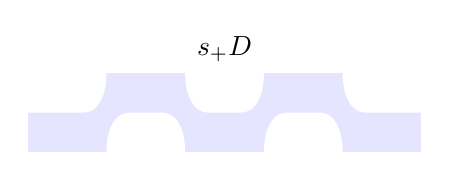
\begin{tikzpicture}[baseline=-0.65ex,scale=0.10]
        \node at (0, 8) {$s_+D$};
        \draw[fill=blue!10!white,draw=none] (-25, -5) rectangle (25, 5);
        \draw[fill=white, draw=none] (-15, -5) [in=left, out=up] to (-12, 0) -- (-8, 0) [in=up, out=right] to (-5, -5);
        \draw[fill=white, draw=none] (5, -5) [in=left, out=up] to (8, 0) -- (12, 0) [in=up, out=right] to (15, -5);
        \draw[fill=white, draw=none] (-5, 5) [in=left, out=down] to (-2, 0) -- (2, 0) [in=down, out=right] to (5, 5);
        \draw[fill=white, draw=none] (-25, 0) -- (-18, 0) [in=down, out=right] to (-15, 5) -- (-25, 5);
        \draw[fill=white, draw=none] ( 25, 0) -- ( 18, 0) [in=down, out=left] to ( 15, 5) -- ( 25, 5);
    \end{tikzpicture}
    \quad
    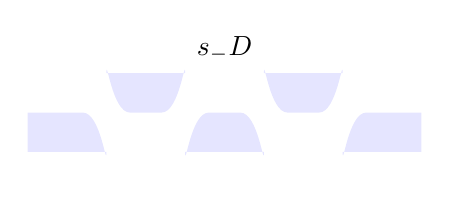
\begin{tikzpicture}[baseline=-0.65ex,scale=0.10]
        \node at (0, 8) {$s_-D$};
        \draw[fill=blue!10!white, draw=none] (-15, 5) [in=left, out=up] to (-12, 0) -- (-8, 0) [in=up, out=right] to (-5, 5);
        \draw[fill=blue!10!white, draw=none] (5, 5) [in=left, out=up] to (8, 0) -- (12, 0) [in=up, out=right] to (15, 5);
        \draw[fill=blue!10!white, draw=none] (-5, -5) [in=left, out=down] to (-2, 0) -- (2, 0) [in=down, out=right] to (5, -5);
        \draw[fill=blue!10!white, draw=none] (-25, 0) -- (-18, 0) [in=down, out=right] to (-15, -5) -- (-25, -5);
        \draw[fill=blue!10!white, draw=none] ( 25, 0) -- ( 18, 0) [in=down, out=left] to ( 15, -5) -- ( 25, -5);
    \end{tikzpicture}
\]

Zamknięte krzywe tworzące $s_+D$ są brzegami białych obszarów uszachowienia,
podczas gdy te tworzące $s_-D$ stanowią brzeg czarnych obszarów.
Zauważmy jeszcze, że na każdym skrzyżowaniu są cztery różne czarne i~białe obszary
(nie mogą się spotkać w~innych miejscach), gdyż diagram był zredukowany.

\begin{lemma}
    \label{lem:pretait_lemma_1}
    Niech $D$ będzie spójnym diagramem splotu o~$n$ skrzyżowaniach.
    Wtedy
    \begin{equation}
        |s_+D| + |s_-D| \le n+2,
    \end{equation}
    z~równością gdy diagram $D$ jest alternujący i~zredukowany.
\end{lemma}

\begin{proof}
    Skorzystamy z~indukcji względem $n$.
    Łatwo widać prawdziwość lematu dla $n = 0$.
    Załóżmy, że jest on prawdziwy dla wszystkich diagramów o~$n - 1$ skrzyżowaniach, następnie ustalmy diagram $D$ o~$n$ skrzyżowaniach.

    Wybierzmy skrzyżowanie z~$D$. Można je wygładzić na dwa sposoby, jeden z~nich daje spójny diagram $D'$.
    Bez straty ogólności przyjmijmy, że jest to dodatnie wygładzenie.
    Wtedy zachodzi $|s_+D'| = |s_+D|$, ale $|s_-D'|=|s_-D|\pm 1$, ponieważ $s_-D'$ powstaje z~$s_-D$ przez zastąpienie pewnej części
    $\LittleRightSmoothing$ z~$\LittleLeftSmoothing$.
    To rozrywa jedną krzywą na dwa kawałki lub scala dwie krzywe w~jedną.
    Teraz z założenia indukcyjnego wynika
    \begin{align}
        |s_+D| + |s_-D|
        & = |s_+D'| + |s_-D'| \pm 1 \\
        & \le (n - 1) + 2 \pm 1 \\
        & \le n + 2.
    \end{align}

    Załóżmy, że $D$ jest spójny, alternujący oraz zredukowany.
    Musimy pokazać, że ostatnie dwie nierówności tak naprawdę są równościami.
    Pierwsza wynika z~tego, że $D'$ jest spójny, alternujący i~zredukowany.
    Z drugiej strony $|s_-D'|=|s_-D|-1$, ponieważ przejście od $s_-D$ do $s_-D'$ skleja dwa czarne obszary, jak na poniższym rysunku:
    \[
        \begin{tikzpicture}[baseline=-0.65ex,scale=0.20]
        \begin{knot}[clip width=5]
            \strand[semithick] (-5, 0) to (5, 0);
            \strand[semithick] (0, -5) to (0, 5);
            \draw[fill=blue!10!white,draw=none] (-5, -5) rectangle (0, 0);
            \draw[fill=blue!10!white,draw=none] ( 5,  5) rectangle (0, 0);
            \node at (0, -8) {$D$};
        \end{knot}
        \end{tikzpicture}
        \quad
        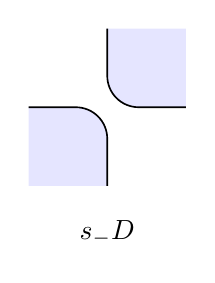
\begin{tikzpicture}[baseline=-0.65ex,scale=0.20]
            \draw[fill=blue!10!white, draw=none] (-5, 0) -- (-2, 0) [in=up, out=right] to (0, -2) -- (0, -5) -- (-5, -5);
            \draw[fill=blue!10!white, draw=none] (5, 0) -- (2, 0) [in=down, out=left] to (0, 2) -- (0, 5) -- (5, 5);
            \draw[semithick] (-5, 0) -- (-2, 0) [in=up, out=right] to (0, -2) -- (0, -5);
            \draw[semithick] (5, 0) -- (2, 0) [in=down, out=left] to (0, 2) -- (0, 5);
            \node at (0, -8) {$s_-D$};
        \end{tikzpicture}
        \quad
        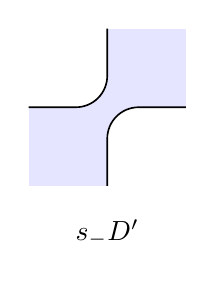
\begin{tikzpicture}[baseline=-0.65ex,scale=0.20]
            \draw[fill=blue!10!white, draw=none] (-5, -5) rectangle (5, 5);
            \draw[fill=white, draw=none] (5, 0) -- (2, 0) [in=up, out=left] to (0, -2) -- (0, -5) -- (5, -5);
            \draw[fill=white, draw=none] (-5, 0) -- (-2, 0) [in=down, out=right] to (0, 2) -- (0, 5) -- (-5, 5);
            \draw[semithick] (5, 0) -- (2, 0) [in=up, out=left] to (0, -2) -- (0, -5);
            \draw[semithick] (-5, 0) -- (-2, 0) [in=down, out=right] to (0, 2) -- (0, 5);
            \node at (0, -8) {$s_-D'$};
        \end{tikzpicture}
        \qedhere
    \]
    To kończy dowód.
    \end{proof}

 \begin{lemma}
    \label{lem:pretait_lemma_2}
    Niech $D$ będzie diagramem splotu o~$n$ skrzyżowaniach.
    Wtedy
    \begin{align}
        M \langle D & \rangle \le n + 2|s_+D| - 2 \\
        m \langle D & \rangle \ge -n - 2|s_-D| + 2
    \end{align}
    z równością, jeżeli $D$ jest alternujący, zredukowany i~spójny.
\end{lemma}

\begin{proof}
    Udowodnimy tylko pierwszą część, druga jest do niej podobna.

    Niech $s$ będzie dowolnym stanem.
    Zauważmy, że $M \langle D|s\rangle = 2|sD| + |s| - 2$, a więc w~szczególności $M \langle D|s_+\rangle = 2|s_+D| + n - 2$.
    Gdyby udało się nam pokazać nierówność $M\langle D|s\rangle \le M\langle D|s_+\rangle$
    dla wszystkich innych stanów $s$, dowód lematu byłby zakończony.

    Kolejną ważną obserwacją jest to, że istnieje ciąg stanów $s_+ = s_0$, $s_1$, \ldots, $s_r=s$, w którym $s_{i+1}$ powstaje z~$s_i$ przez pojedynczą zmianę $+1$ na $-1$.
    Diagram $s_{i+1}D$ uzyskujemy z~$s_{i}D$ przez połączenie dwóch zamkniętych krzywych lub podział jednej zamkniętej krzywej na dwie części.
    Wynikają stąd równości $|s_{i+1}| = |s_i| - 2$ oraz $|s_{i+1}D| = |s_iD| \pm 1$.
    To kończy dowód nierówności z lematu, ponieważ
    \begin{align}
        M \langle D \mid s_{i+1} \rangle
        & = 2|s_{i+1}D| + |s_{i+1}|-2 \\
        & = (2|s_iD| + |s_i| -2 ) + (\pm 2-2) \\
        & \le M \langle D|s_i\rangle.
    \end{align}
    Powtarzając odpowiednio wiele razy dostajemy łańcuch nierówności
    \begin{equation}
        \langle D \mid s\rangle =M\langle D \mid s_r\rangle \le\ldots\le M\langle D \mid s_0\rangle=M\langle D \mid s_+\rangle
    \end{equation}

    Pokażemy teraz, że jeśli $D$ jest zredukowany, alternujący i~spójny, to nierówność zamienia się w~równość.
    Będzie to wynikało z ostrej nierówności
    \begin{equation}
        M\langle D|s\rangle < M\langle D| s_+\rangle
    \end{equation}
    dla $s\neq s_+$, jeżeli tylko powołamy się na powyższy argument.
    Wystarczy ograniczyć się do tych $s$, które powstają z~$s_+$ przez zmianę pojedynczego stanu $+1$ na $-1$.
    Ale to już jest oczywiste, gdyż $sD$ otrzymujemy przez sklejenie dwóch białych obszarów $s_+ D$.
\end{proof}

Możemy wreszcie zająć się rozpiętością wielomianu Jonesa.

\begin{proposition}
    Niech $L$ będzie zorientowanym splotem o~spójnym diagramie $D$ z~$n$ skrzyżowaniami.
    Wtedy $\operatorname{span} \jones(L) \le n$, z~równością dla zredukowanego i~alternującego $D$.
\end{proposition}

\begin{proof}
    Pokażemy prawdziwość innego, równoważnego stwierdzenia: $\operatorname{span} \langle D\rangle\le 4n$.
    Dwa poprzednie lematy \ref{lem:pretait_lemma_1} oraz \ref{lem:pretait_lemma_2} raze, mówią, że
    \begin{align}
        \operatorname{span}\langle D\rangle
        & = M\langle D\rangle - m\langle D\rangle \\
        & \le (2|s_+D|+n-2)+(2|s_-D|+n-2) \\
        & = 2(|s_+D|+|s_- D|)+2n-4 \\
        & \le 2(n+2)+2n-4 \\
        & = 4n. \qedhere
    \end{align}
\end{proof}

Jesteśmy już w~stanie podać dowód twierdzenia \ref{taitjones} wspomnianego na początku sekcji.

\begin{proof}
    Założenia mówią nam, że $\operatorname{span} (\jones(L)) = n$.
    Gdyby istniał diagram o~mniejszej liczbie skrzyżowań,
    mielibyśmy $\operatorname{span} (\jones(L)) < n$, co prowadzi do sprzeczności.
\end{proof}

Szukanie wielomianu Jonesa splotu bywa uciążliwe,
jednak czasami możemy oszacować jego rozpiętość korzystając z~następujących nierówności:

\begin{corollary}
    Niech $L$ będzie zorientowanym splotem ze spójnym diagramem $D$ o~$n$ skrzyżowaniach.
    Wtedy
    \begin{align}
        3w(D)-2|s_+D|+2-n & \le 4 m(\jones(L) \\
        3w(D)+2|s_-D|+n-2 & \ge 4 M(\jones(L)),
    \end{align}
    z~równością dla zredukowanego i~alternującego $D$.
\end{corollary}

\begin{proof}
    Wystarczy powołać się na definicję \ref{def:jones_polynomial} oraz lemat \ref{lem:pretait_lemma_2}.
\end{proof}

% Koniec podsekcji Rozpiętość i~wielomian Jonesa


\subsection{Definicja algebraiczna -- algebra Temperleya-Lieba} % (fold)
\label{sub:jones_paper}
Jones otrzymał swój wielomian jako efekt uboczny badań nad algebrami operatorowymi: wziął ślad pewnej reprezentacji warkoczy w~algebrę, która miała ważne znaczenie w~mechanice statystycznej.
Dalszy opis pochodzi z Wikipedii.
Zaletą tego podejścia jest możliwość wyboru algebry, która reprezentuje grupę warkoczy.

\begin{definition}[algebra Temperleya-Lieba]
    Niech $R$ będzie przemiennym pierścieniem, w~którym ustalono element $\delta \in R$.
    Wtedy $R$-algebrę $TL_n(\delta)$ generowaną przez elementy $e_1, \ldots, e_{n-1}$, które związane są relacjami
    \begin{align}
        e_i^2 & = \delta e_i, \\
        e_i e_{i \pm 1} e_i & = e_i, \\
        e_i e_j & = e_j e_i
    \end{align}
    dla $|i-j| \ge 2$, nazywamy algebrą Temperleya-Lieba.
    % Algebra Temperleya-Lieba $A_n$ to wolna addytywna algebra na multiplikatywnych generatorach $e_1, \ldots, e_{n-1}$ traktowana jako $\C[\tau, \tau^{-1}]$-moduł.
    % Zmienna $\tau$ komutuje ze wszystkimi generatorami, generatory zaś spełniają relacje ($j$ jest różne od $i - 1, i, i+1$):
\end{definition}

$TL_n(\delta)$ można przedstawić przy użyciu diagramów: prostokątów, których przeciwległe boki zawierają po $n$ punktów połączonych w~pary tak, by uniknąć samoprzecięć. Mnożenie elementów algebry odpowiada sklejaniu dwóch diagramów, przy czym każdą zamkniętą pętlę zamieniamy na dodatkowy czynnik $\delta$.
To w~gruncie rzeczy są warkocze.

\begin{definition}[ślad Markowa]
    Niech $K \in TL_n(\delta)$ będzie elementem algebry Temperleya-Lieba będącym iloczynem generatorów\footnote{Czyli element $K$ utożsamia się z~pewnym warkoczem o~$n$ pasmach.} $e_1, \ldots, e_{n-1}$, którego domknięcie rozpada się na $m$ składowych spójności.
    Śladem Markowa elementu $K$ nazywamy wielkość $\operatorname{tr} K = \delta^{m-n}$.
\end{definition}

Na mocy twierdzenia Alexandera, każdy splot $L$ jest domknięciem warkocza zaplecionego na pewnej liczbie pasm.
Zdefiniujmy reprezentację $\rho \colon B_n \to TL_n$ grupy warkoczy w~algebrę Temperleya-Lieba związaną z pierścieniem $R = \Z[A, 1/A]$ oraz elementem $\delta = -A^2 - A^{-2}$ wzorem
\begin{equation}
    \rho(\sigma_i) = A \cdot e_i + \frac{1}{A} \cdot 1.
\end{equation}
Wtedy $\langle K \rangle = \delta^{n-1} \operatorname{tr} \rho (\sigma)$ jest klamrą Kauffmana.
Pozostaje sprawdzić wpływ ruchów Markowa na złożenie $\operatorname{tr} \circ \rho$, ponieważ sploty nie przedstawiają się jako domknięcia warkoczy jednoznacznie.

% Koniec podsekcji Oryginalna praca Jonesa


\begin{proposition}
\label{prp:jones_trivial_link}
    Wielomianem Jonesa splotu trywialnego jest $V(K_n) = (-1)^{n-1} (\sqrt{t} - 1/\sqrt{t})^{n-1}$.
\end{proposition}

% Koniec sekcji Wielomian Jonesa